\documentclass[14pt, aspectratio=169]{beamer}
\usepackage[T1]{fontenc}
\usepackage[english]{babel} % german as language
\usepackage{csquotes}
\usepackage{parskip} % for paragraph line skip

% for tables/figures
\usepackage{graphicx}
\usepackage{caption}
\usepackage{array}
\graphicspath{ {figures/} } % set path to figures
\renewcommand{\listfigurename}{Abbildungsverzeichnis}
\renewcommand{\listtablename}{Tabellenverzeichnis}

% Appendix
\usepackage[toc,page]{appendix}
\renewcommand\appendixname{Anhang} % Change name to German
\renewcommand\appendixpagename{Anhang}
\renewcommand\appendixtocname{Anhang}


% \usepackage{sectsty} -> falls section font size 14 haben muss
% \sectionfont{\large\bfseries}


% Citation: BibLaTeX als author-year style, benötigt xelatex->biber->xelatex(2x) als recipe!
\usepackage[
backend=biber,
style=authoryear]{biblatex}
\addbibresource{refs.bib}

% Titel/Startseite
\title{AI Generated Texts in Higher Education}
\author{Lukas Schaffrath}
\date{December 2025}

%theme
%%general
\usetheme[right]{PaloAlto}
\setbeamersize{text margin left=1em, text margin right=1em}

%%catpuccin
\definecolor{ctpRosewater}{HTML}{F5E0DC}
\definecolor{ctpFlamingo}{HTML}{F2CDCD}
\definecolor{ctpPink}{HTML}{F5C2E7}
\definecolor{ctpMauve}{HTML}{CBA6F7}
\definecolor{ctpRed}{HTML}{F38BA8}
\definecolor{ctpMaroon}{HTML}{EBA0AC}
\definecolor{ctpPeach}{HTML}{FAB387}
\definecolor{ctpYellow}{HTML}{F9E2AF}
\definecolor{ctpGreen}{HTML}{A6E3A1}
\definecolor{ctpTeal}{HTML}{94E2D5}
\definecolor{ctpSky}{HTML}{89DCEB}
\definecolor{ctpSapphire}{HTML}{74C7EC}
\definecolor{ctpBlue}{HTML}{89B4FA}
\definecolor{ctpLavender}{HTML}{B4BEFE}
\definecolor{ctpText}{HTML}{CDD6F4}
\definecolor{ctpSubtext1}{HTML}{BAC2DE}
\definecolor{ctpSubtext0}{HTML}{A6ADC8}
\definecolor{ctpOverlay2}{HTML}{9399B2}
\definecolor{ctpOverlay1}{HTML}{7F849C}
\definecolor{ctpOverlay0}{HTML}{6C7086}
\definecolor{ctpSurface2}{HTML}{585B70}
\definecolor{ctpSurface1}{HTML}{45475A}
\definecolor{ctpSurface0}{HTML}{313244}
\definecolor{ctpBase}{HTML}{1E1E2E}
\definecolor{ctpMantle}{HTML}{181825}
\definecolor{ctpCrust}{HTML}{11111B}

% Main colors
\setbeamercolor{background canvas}{bg=ctpBase}
\setbeamercolor{normal text}{fg=ctpText,bg=ctpBase}
\setbeamercolor{frametitle}{fg=ctpMauve,bg=ctpBase}
\setbeamercolor{title}{fg=ctpBlue,bg=ctpBase}
\setbeamercolor{author}{fg=ctpText}
\setbeamercolor{date}{fg=ctpSubtext1}
\setbeamercolor{section in toc}{fg=ctpMauve}
\setbeamercolor{structure}{fg=ctpMauve}

% Items
\setbeamercolor{itemize item}{fg=ctpLavender}
\setbeamercolor{itemize subitem}{fg=ctpSapphire}
\setbeamercolor{enumerate item}{fg=ctpLavender}

% Blocks
\setbeamercolor{block title}{fg=ctpYellow,bg=ctpSurface1}
\setbeamercolor{block body}{fg=ctpText,bg=ctpSurface0}

% Buttons and links
\setbeamercolor{button}{bg=ctpBlue,fg=ctpBase}
\hypersetup{
    colorlinks=true,
    linkcolor=ctpSky,
    urlcolor=ctpTeal
}

% Sidebar colors
\setbeamercolor{sidebar}{bg=ctpSurface0}
\setbeamercolor{sidebar right}{bg=ctpSurface0}
\setbeamercolor{title in sidebar}{fg=ctpSky}
\setbeamercolor{author in sidebar}{fg=ctpSubtext1}
\setbeamercolor{section in sidebar}{fg=ctpText,bg=ctpSurface1}
\setbeamercolor{section in sidebar shaded}{fg=ctpSubtext1,bg=ctpSurface0}
\setbeamercolor{subsection in sidebar}{fg=ctpSapphire}
\setbeamercolor{subsection in sidebar shaded}{fg=ctpOverlay1}

% Palette colors
\setbeamercolor{palette sidebar primary}{fg=ctpSky,bg=ctpSurface0}
\setbeamercolor{palette sidebar secondary}{fg=ctpMauve,bg=ctpSurface0}
\setbeamercolor{palette sidebar tertiary}{fg=ctpText,bg=ctpSurface0}
\setbeamercolor{palette sidebar quaternary}{fg=ctpSubtext1,bg=ctpSurface0}

% Headline (die Box oben) - dunkler Hintergrund
\setbeamercolor{section in head/foot}{fg=ctpMauve,bg=ctpSurface1}
\setbeamercolor{subsection in head/foot}{fg=ctpText,bg=ctpSurface1}

% Templates
\setbeamertemplate{navigation symbols}{}
\setbeamertemplate{frametitle continuation}{}
\setbeamertemplate{section in sidebar shaded}[default]

% Frame-Titel kleiner machen
\setbeamerfont{frametitle}{size=\large}

\makeatletter
\setbeamertemplate{headline}{%
  \ifnum\theframenumber=1\relax
    % Auf Titelseite: keine Headline
  \else
    % Auf anderen Seiten: Frame-Titel anzeigen
    \begin{beamercolorbox}[wd=\paperwidth,ht=4ex,dp=2ex,leftskip=1em]{section in head/foot}
      \usebeamerfont{section in head/foot}\insertframetitle
    \end{beamercolorbox}
  \fi
}
\makeatother

% make each text appear after another!!
\beamerdefaultoverlayspecification{<+->}

% Start des Dokuments
\begin{document}

%Erstelle Titelseite
\maketitle

\section{Background}
\begin{frame}{Background}
    \begin{itemize}
      \pause
      \item Idea: building upon research found in recommended overview papers
      \item Myself: background in teaching (Teacher Trainee B.A./M.Ed.)
      \item AI is a continuous problem in education, as indicated in paper
      \item AI detection is very problematic!
    \end{itemize}
\end{frame}


\begin{frame}{Background}
    \begin{center}
    \textbf{In recommended paper:} \\
    \pause
    Teacher Trainees and teachers trying to recognize AI generated texts\\
    (but failing!)\\
    \vspace{0.5cm}
    \pause
    -> up to now: just teachers/papers to help overcome being detected (see PopAI, 2025)
    \end{center}
\end{frame}

\begin{frame}{Background}
    \begin{center}
      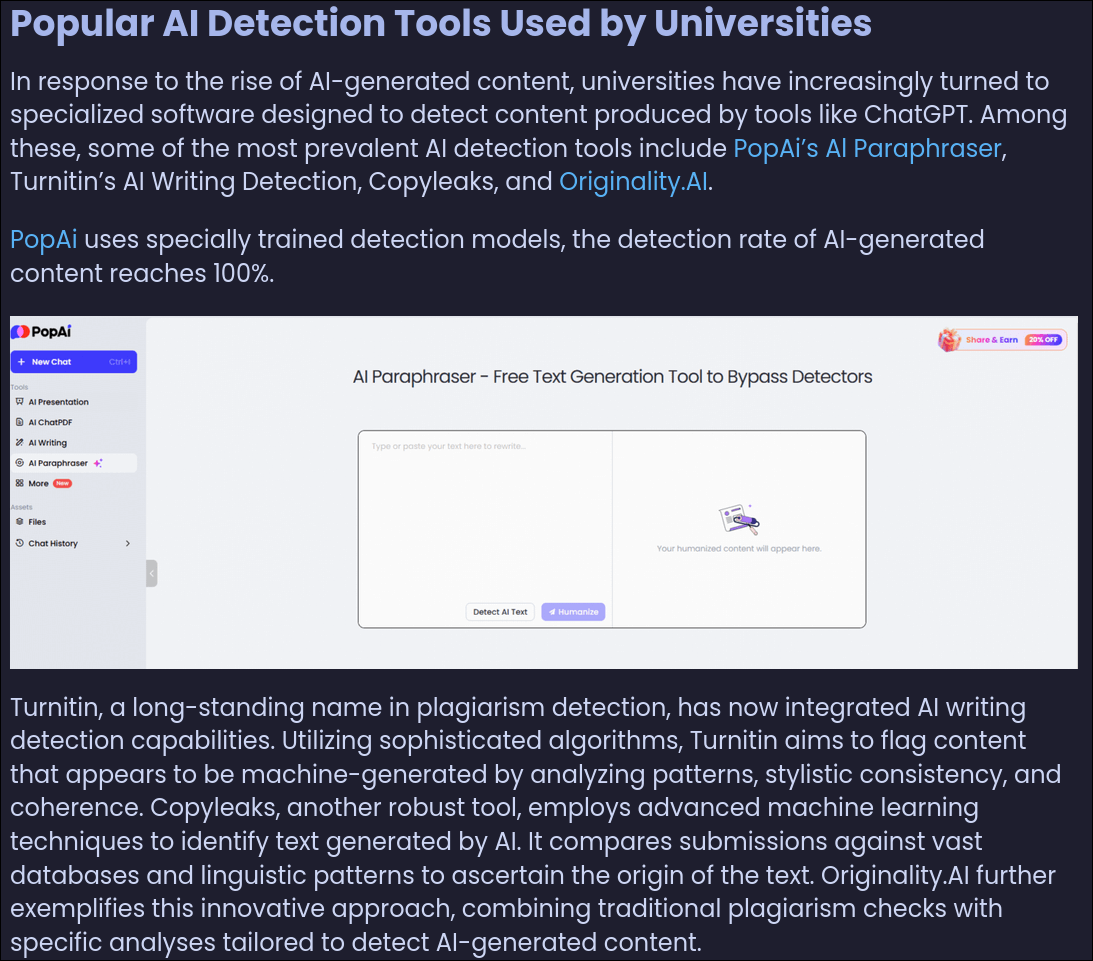
\includegraphics[scale=0.2]{popai.png}\\
      \begin{tiny}
       https://www.popai.pro/resources/can-professors-detect-chatgpt-generated-content/
      \end{tiny}
    \end{center}
\end{frame}

\begin{frame}{Background}
    \begin{center}
    \textbf{Prof. Sven Strasen:}\\
    \vspace{0.5cm}
    \pause
    \textbf{"The characteristics of Chat GPT generated texts are hard to miss"} \\
    \vspace{0.5cm}
    \begin{tiny}
    (Mail from 10/10/25 on term papers in Literary Studies)\\
    \end{tiny}
    \vspace{0.5cm}
    \begin{small}
      \pause
    (He's probably right, but let's see!)
    \end{small}
    \end{center}
\end{frame}


\section{Topic}
\begin{frame}{My Topic}
  \textbf{Do University Instructors Spot AI?: Investigating the Detectability of AI-Generated Student Writing in Higher Education}\\
  \vspace {0.5cm}
  \pause
  \textbf{RQ: To what extent can university instructors distinguish between AI-generated and human-written student texts?}
\end{frame}

\begin{frame}{My Topic}
  \begin{columns}[T]
    \column{0.5\textwidth}
    \textbf{H0:}\\
    \begin{small}
      University instructors cannot distinguish between AI-generated and human-written student texts (i.e., their accuracy rate does not differ significantly from 50\%).
    \end{small}
    \column{0.5\textwidth}
    \textbf{H1:}\\
    \begin{small}
      University instructors can distinguish between AI-generated and human-written student texts(i.e., their accuracy rate is significantly higher than 50\%).
    \end{small}
  \end{columns}
\end{frame}

\section{Operationalization}
\begin{frame}{Operationalization}
\begin{itemize}
  \item 10 texts (5 human/5 AI generated)
  \item Texts from previous student assignments (with permission) (submitted via google forms)
  \item Using a website to collect data
  \item Sent to Profs/Instructors, who rate texts (binary)
  \item Data analyzed using Python
\end{itemize}
\end{frame}

\begin{frame}{Operationalization}
  \begin{columns}[T]
    \column{0.5\textwidth}
    \textbf{Website:}\\
    \vspace{0.2cm}
      
\includegraphics[scale=0.1]{sslandingpage.png}\\
      \begin{tiny}
       https://lstoneyy.pythonanywhere.com/
      \end{tiny}
    \column{0.5\textwidth}
    \textbf{Classification:}\\
    \vspace{0.2cm}
      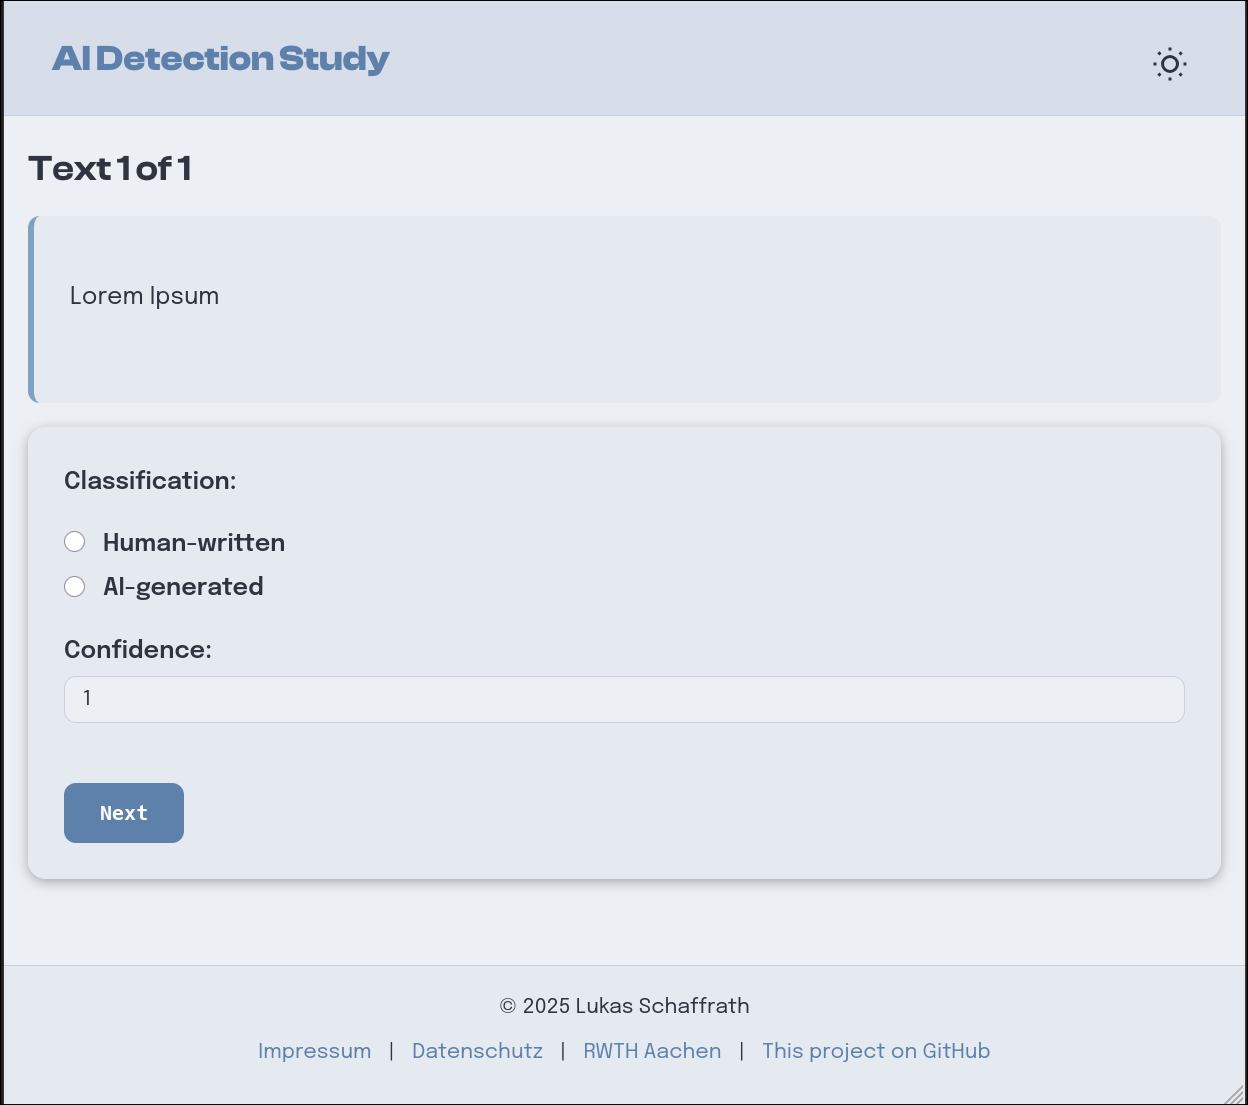
\includegraphics[scale=0.14]{sstextitem.png}\\
  \end{columns}
\end{frame}

\begin{frame}{Operationalization}
    \textbf{Responses}\\
    \vspace{0.2cm}
      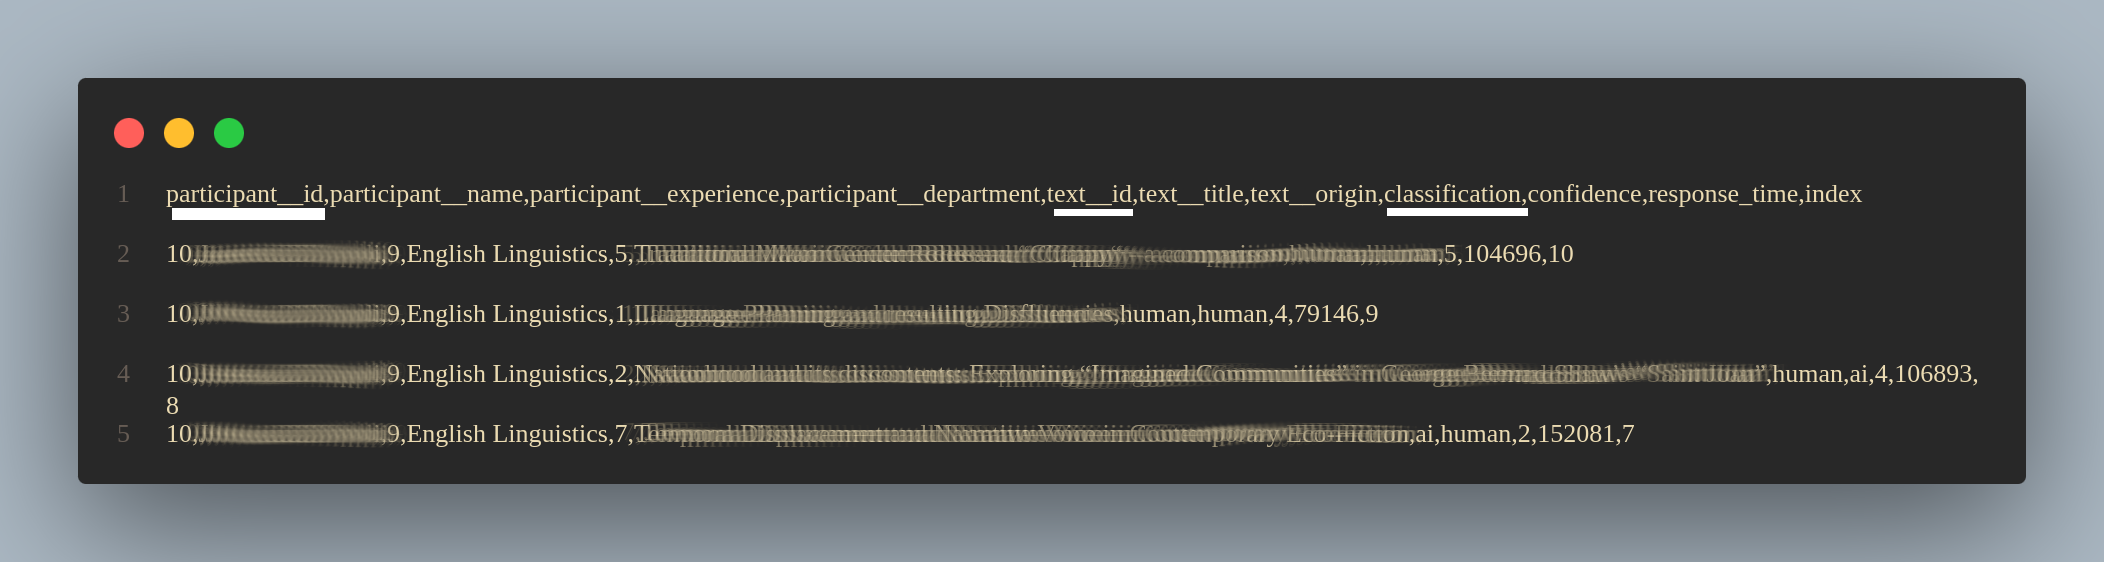
\includegraphics[scale=0.16]{responses.png}\\
      \begin{tiny}
       https://lstoneyy.pythonanywhere.com/
      \end{tiny}
\end{frame}

\begin{frame}{Operationalization}
  \begin{columns}[T]
    \column{0.5\textwidth}
    \textbf{Script}\\
    \vspace{0.2cm}
      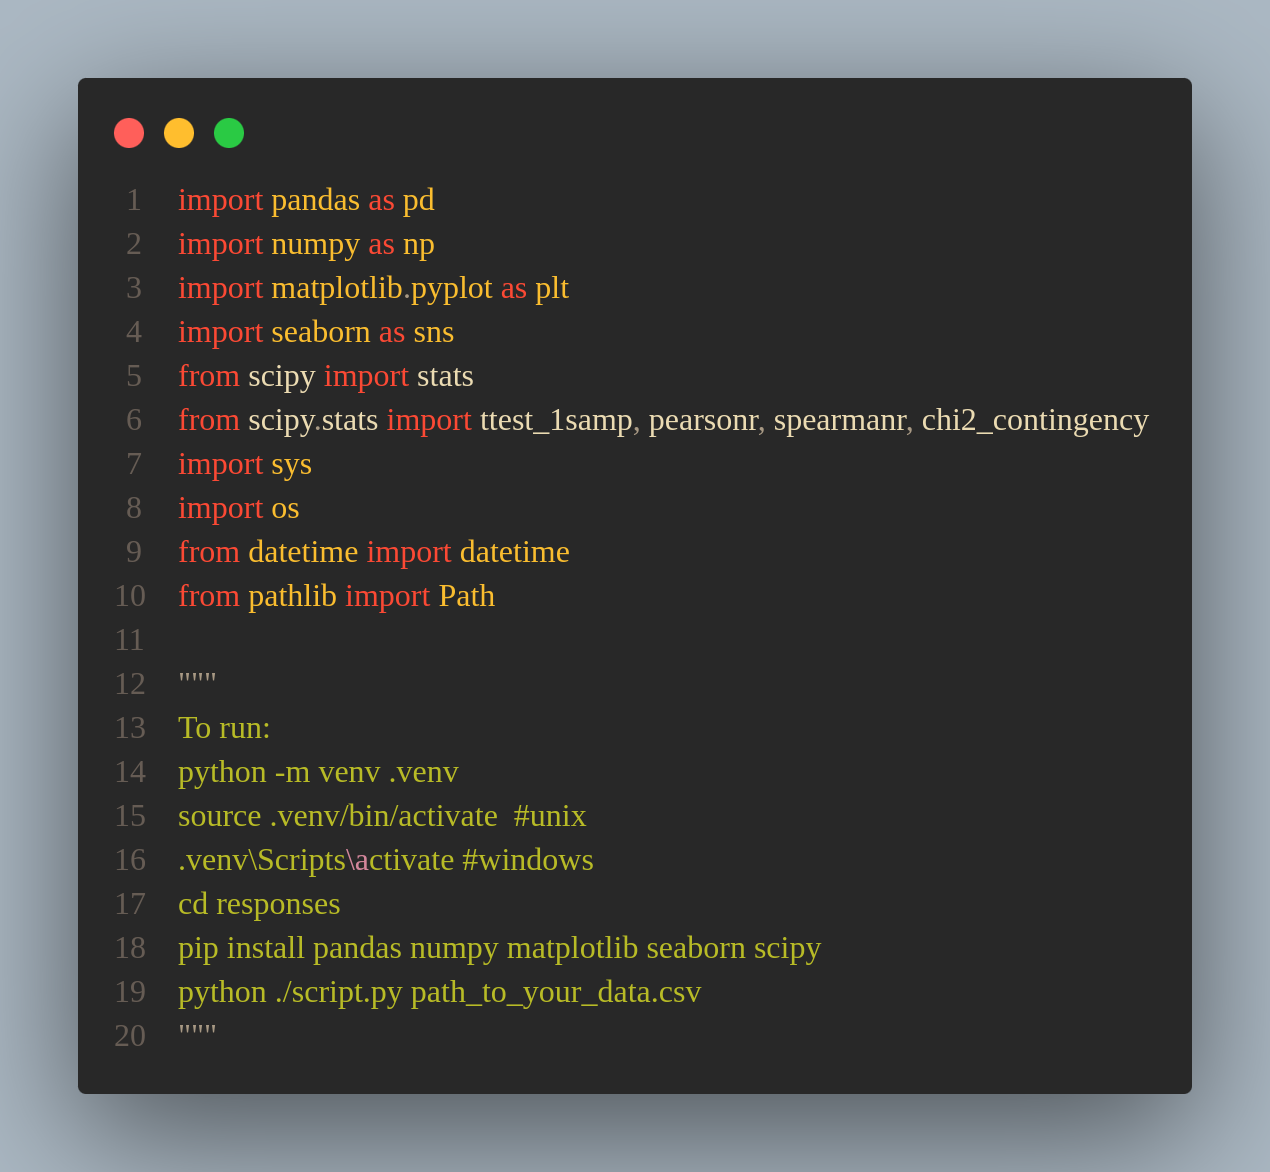
\includegraphics[scale=0.1]{script.png}\\
      \begin{tiny}
       Can be used on any .csv!
      \end{tiny}
    \column{0.5\textwidth}
    \textbf{Output}\\
    \vspace{0.25cm}
      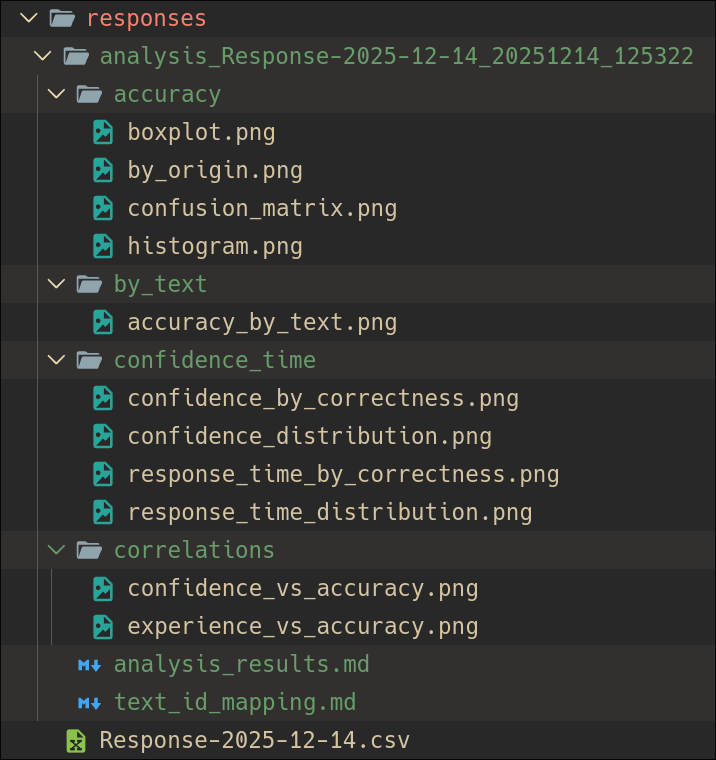
\includegraphics[scale=0.15]{project.png}\\
      \begin{tiny}
       Automatic folder creation with results and plots!
      \end{tiny}
  \end{columns}
\end{frame}

\begin{frame}{Operationalization}
  \begin{columns}[T]
    \column{0.5\textwidth}
    \textbf{Console output}\\
    \vspace{0.2cm}
      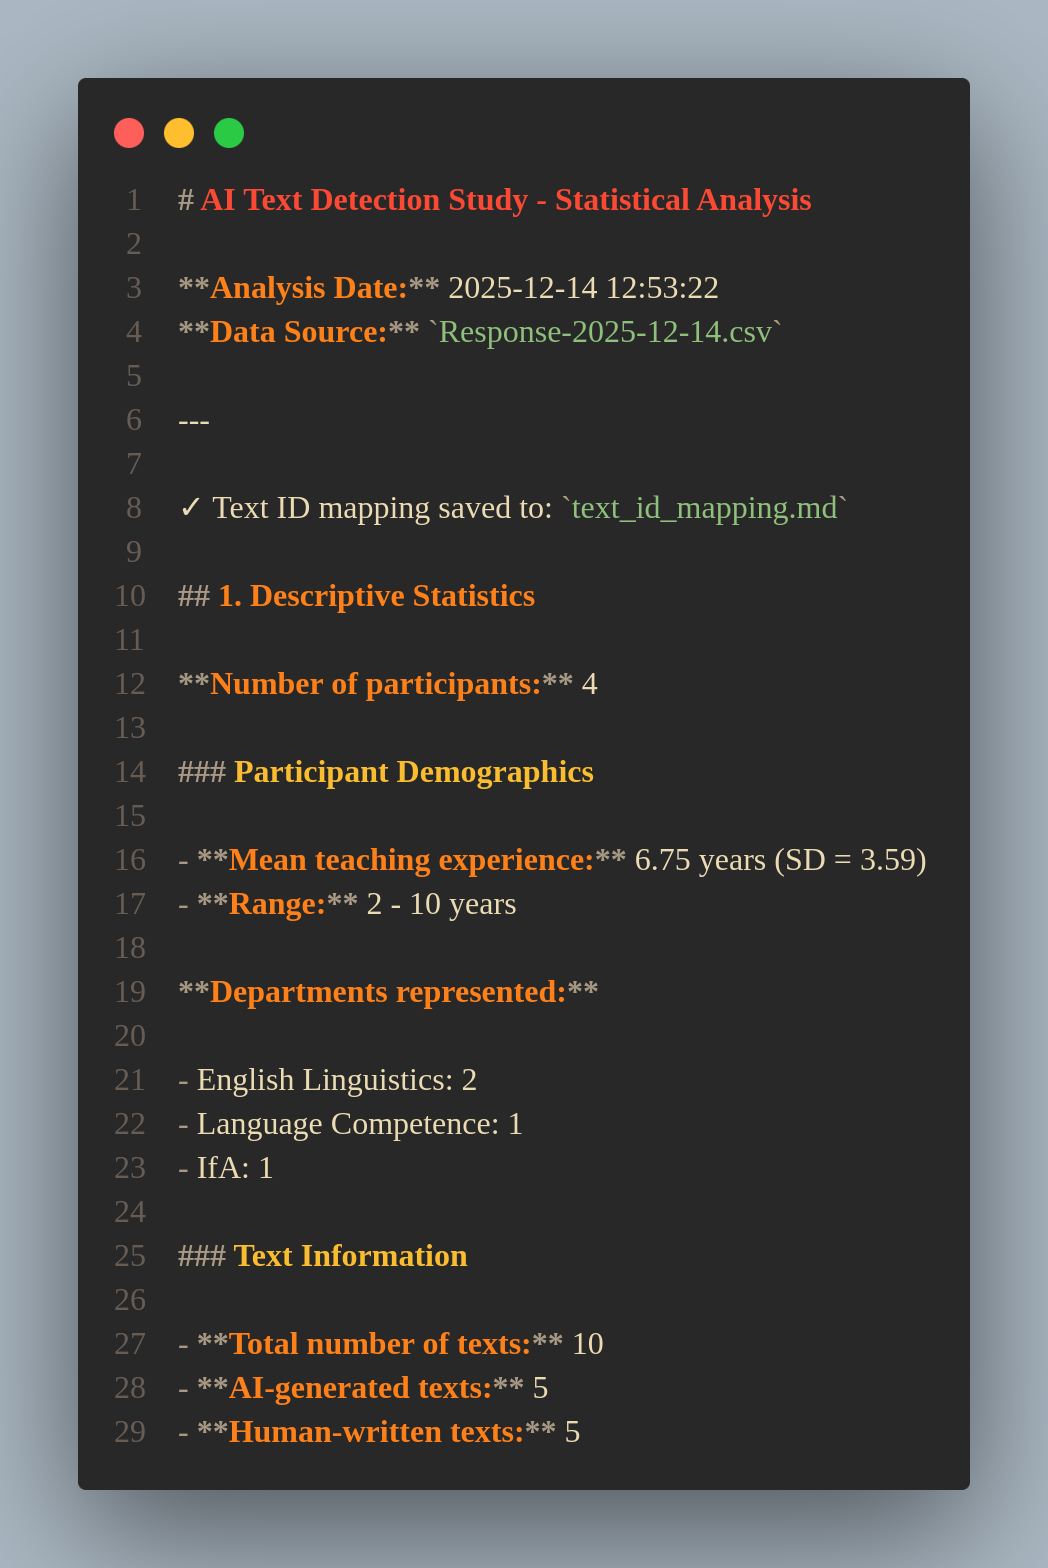
\includegraphics[scale=0.1]{responses1.png}\\
      \begin{tiny}
       Console outputs as Markdown files!
      \end{tiny}
    \column{0.5\textwidth}
    \textbf{Statistics!}\\
    \vspace{0.2cm}
      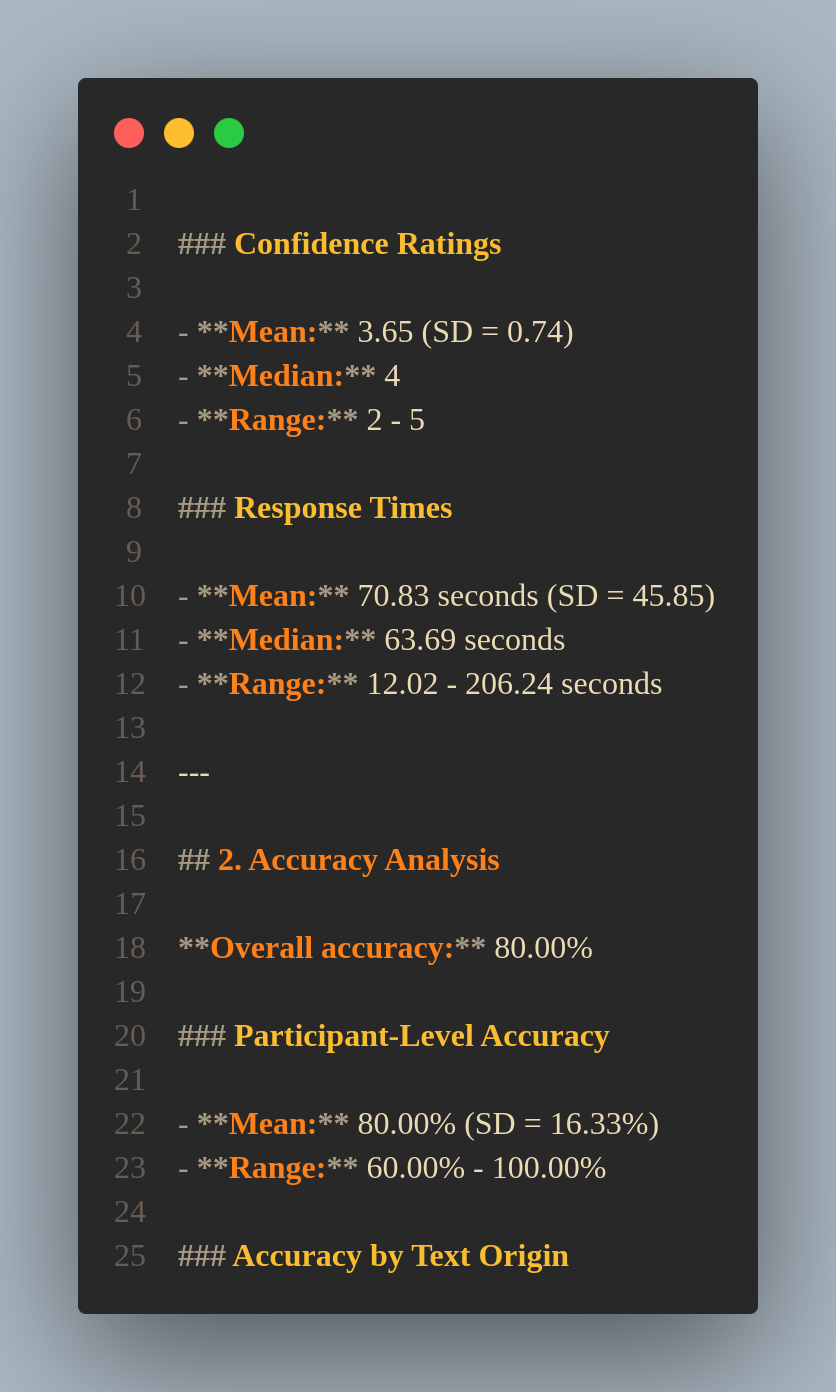
\includegraphics[scale=0.115]{responses2.png}\\
      \begin{tiny}
       File for statistical analysis!
      \end{tiny}
  \end{columns}
\end{frame}

\section{Preliminary Results}
\begin{frame}{Preliminary Results}
\begin{itemize}
  \item Up to now: 4 Participants
  \item Mean teaching experience: 6.75 years
  \item Mean confidence: 3.65/5
  \item Mean response time/text: 70.83 seconds
  \item Overall accuracy: 80\% :
    \begin{itemize}
      \item Human texts: 95\% -> 1 mistake
      \item AI texts: 65\%!! -> 7 mistakes!!
    \end{itemize}
\end{itemize}
\end{frame}

\section{Preliminary Results}
\begin{frame}{Preliminary Results}
    \begin{center}
      \textbf{Interpretation:}\\
      Paritipants performed significantly better than chance, but had difficulties identifying AI-generated texts.
    \end{center}
\end{frame}

\section{Limitations}
\begin{frame}{Limitations}
\begin{itemize}
  \pause
  \item Small sample size (now \& overall!)
  \item Participants mainly from similar fields (all IfAAR)
  \item Text topics from similar fields
  \item No control over external factors (e.g., use of detection tools)
\end{itemize}
\end{frame}

\section{Limitations}
\begin{frame}{Limitations}
\begin{center}
  Results are preliminary;\\
  In future: larger and more diverse samples needed!
\end{center}
\end{frame}

\section{Conclusion}
\begin{frame}{Conclusion}
  \begin{center}
  Thanks for listening :)\\
  \vspace{0.5cm}
  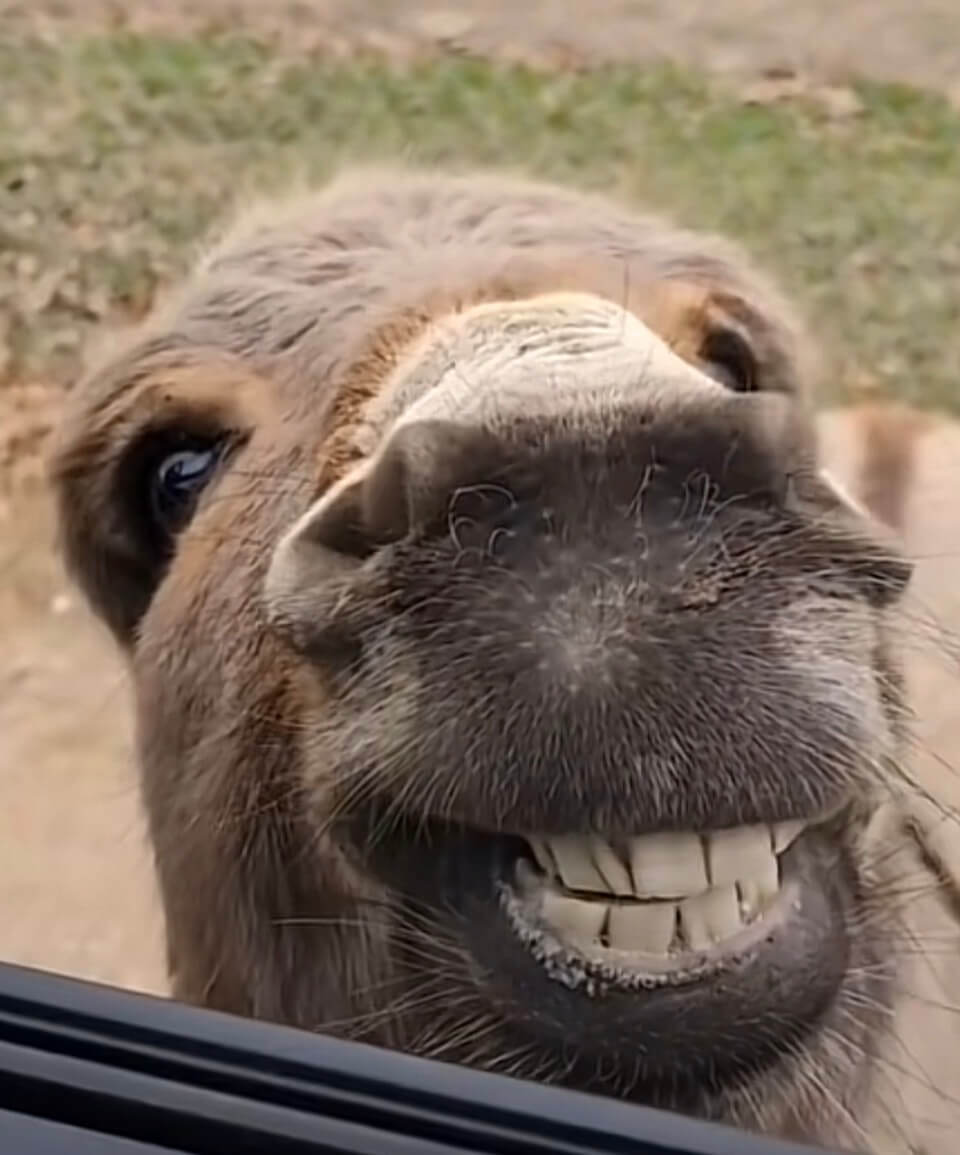
\includegraphics[scale=0.1]{donkey.jpg}
  \end{center}
\end{frame}

\begin{frame}{Conclusion}
  \textbf{Sources}\\
    Fleckenstein, J., Meyer, J., Jansen, T., Keller, S. D., Köller, O., \& Möller, J. (2024). Do teachers spot AI? Evaluating the detectability of AI-generated texts among student essays. Computers \& Education: Artificial Intelligence.
    \begin{tiny}
    https://www.sciencedirect.com/science/article/pii/S2666920X24000109
    \end{tiny}\\
    \vspace{0.2cm}
    PopAI (2025). Can Professors Detect ChatGPT-Generated Content?\\
    \begin{tiny}
    https://www.popai.pro/resources/can-professors-detect-chatgpt-generated-content/
    \end{tiny}\\
\end{frame}

% % Add table of contents with emtpy page number
% \addtocontents{toc}{\protect\thispagestyle{empty}}
% \tableofcontents

% % List of figures and tables
% \newpage
% \thispagestyle{empty}
% \listoffigures
% \vspace{0.5cm}
% \listoftables



% print bibliography with heading in table of contents
% \newpage
% \printbibliography[heading=bibintoc]
% \pagestyle{empty}

\end{document}
